%Following is an open list of problems that we will address in order to achieve device composition by means of implicit interaction.
%\begin{enumerate}
%\item{\emph{Setup}: How is a device enabled for integrating with a tabletop?
%The setup should be simple, to be performed only once by non-technical users.
%An initial survey of possible solutions points towards the use of tagging mechanisms and/or camera-based object recognition.}
%\item{\emph{Discovery}: How do the tabletop and the device discover and communicate with each other?
%How do we solve the issues of discovery, handshake, network connectivity, and encryption mechanisms to ensure privacy?}
%\item{\emph{UI transfer}: Given the computational constraints of mobile devices, how can the UI transfer be efficiently implemented so as to support native applications and guarantee a seamless user experience?}
%\item{\emph{Input}: How can the users interact with their applications on the tabletop (touch and other peripherals)?}
%\item{\emph{Interaction Design}: What means of interaction are best-fitted for the tabletop-based systems that we propose to develop?
%How can we best adapt to public/private uses and single/multiple users?
%How can we take advantage of the larger interaction surface?}
%\end{enumerate}

%%%%%%%%%%%%%%%%%%%%%%
%%% IMPLEMENTATION %%%
%%%%%%%%%%%%%%%%%%%%%%

\chapter{The TIDE prototype}
\label{system}

TIDE (Tabletop Interactive Display Extension) is a prototype that combines smartphones and tabletops by way of UI replication.
It was implemented in .NET for the Microsoft Surface (Windows Vista), referred to as MS in this chapter.
It was tested with an iPhone 4 running iOS 5 and a HTC Legend phone running Google Android 2.1, but it can be extended to support other smartphone models.

As shown in figure~\ref{fig:overview}, TIDE consists of three components, that are responsible for pairing, UI replication, and the surface UI.
Pairing is done through camera-based object detection.
TIDE relies on OpenCV (Open Source Computer Vision) \citep{opencv} to detect phone-like objects to connect to, and to track the devices during the application session.
The UI replication is based on the VNC protocol \citep{Richardson:1998:vnc}.
TIDE includes a VNC client that is based on the VncSharp library \citep{vncsharp}, and that connects over the network to a VNC server running on the smartphone (third-party application).
The surface UI is implemented using the Microsoft Surface SDK and WPF (Windows Presentation Foundations).
\\
\linebreak
Figure~\ref{fig:sequenceOverview} shows the basic interaction flow that TIDE supports.
First, the user places the smartphone the MS, which triggers the pairing process, described in section~\ref{sec:pairing}.
Second, the smartphone's UI is replicated to the tabletop via the VNC protocol, as presented in section~\ref{sec:replicated}.
Lastly, the user interacts with the application via the surface UI, described in section~\ref{sec:surfaceui}.

\begin{figure}[htb]
  \centering
    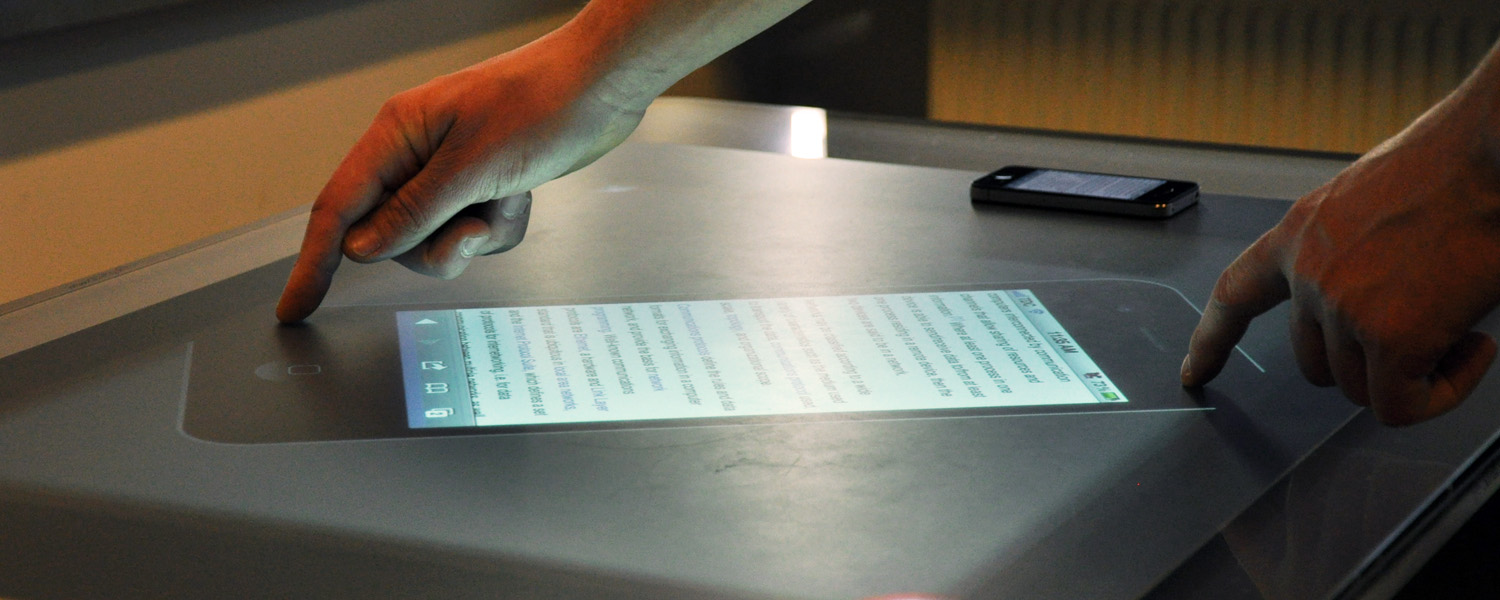
\includegraphics[width=0.8\textwidth]{images/tideHands}
    \caption{The TIDE prototype.}
    \label{fig:tideHands}
\end{figure}

\begin{figure}[htb]
  \centering
    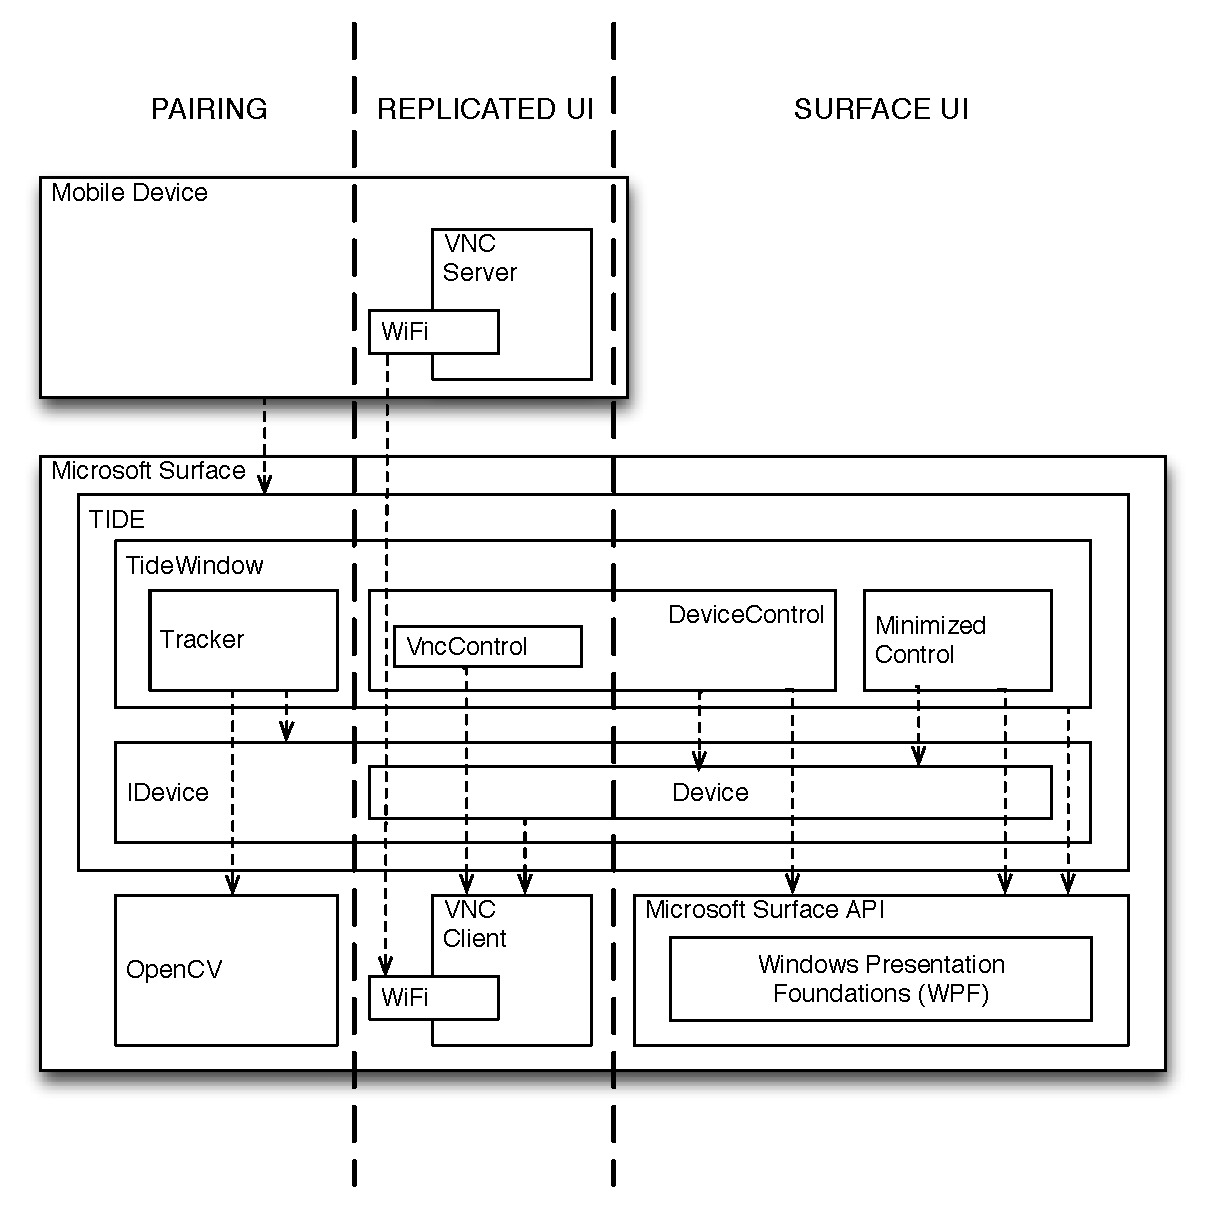
\includegraphics[width=1\textwidth]{images/overview}
    \caption{TIDE overview.}
    \label{fig:overview}
\end{figure}

\begin{figure}[htb]
  \centering
    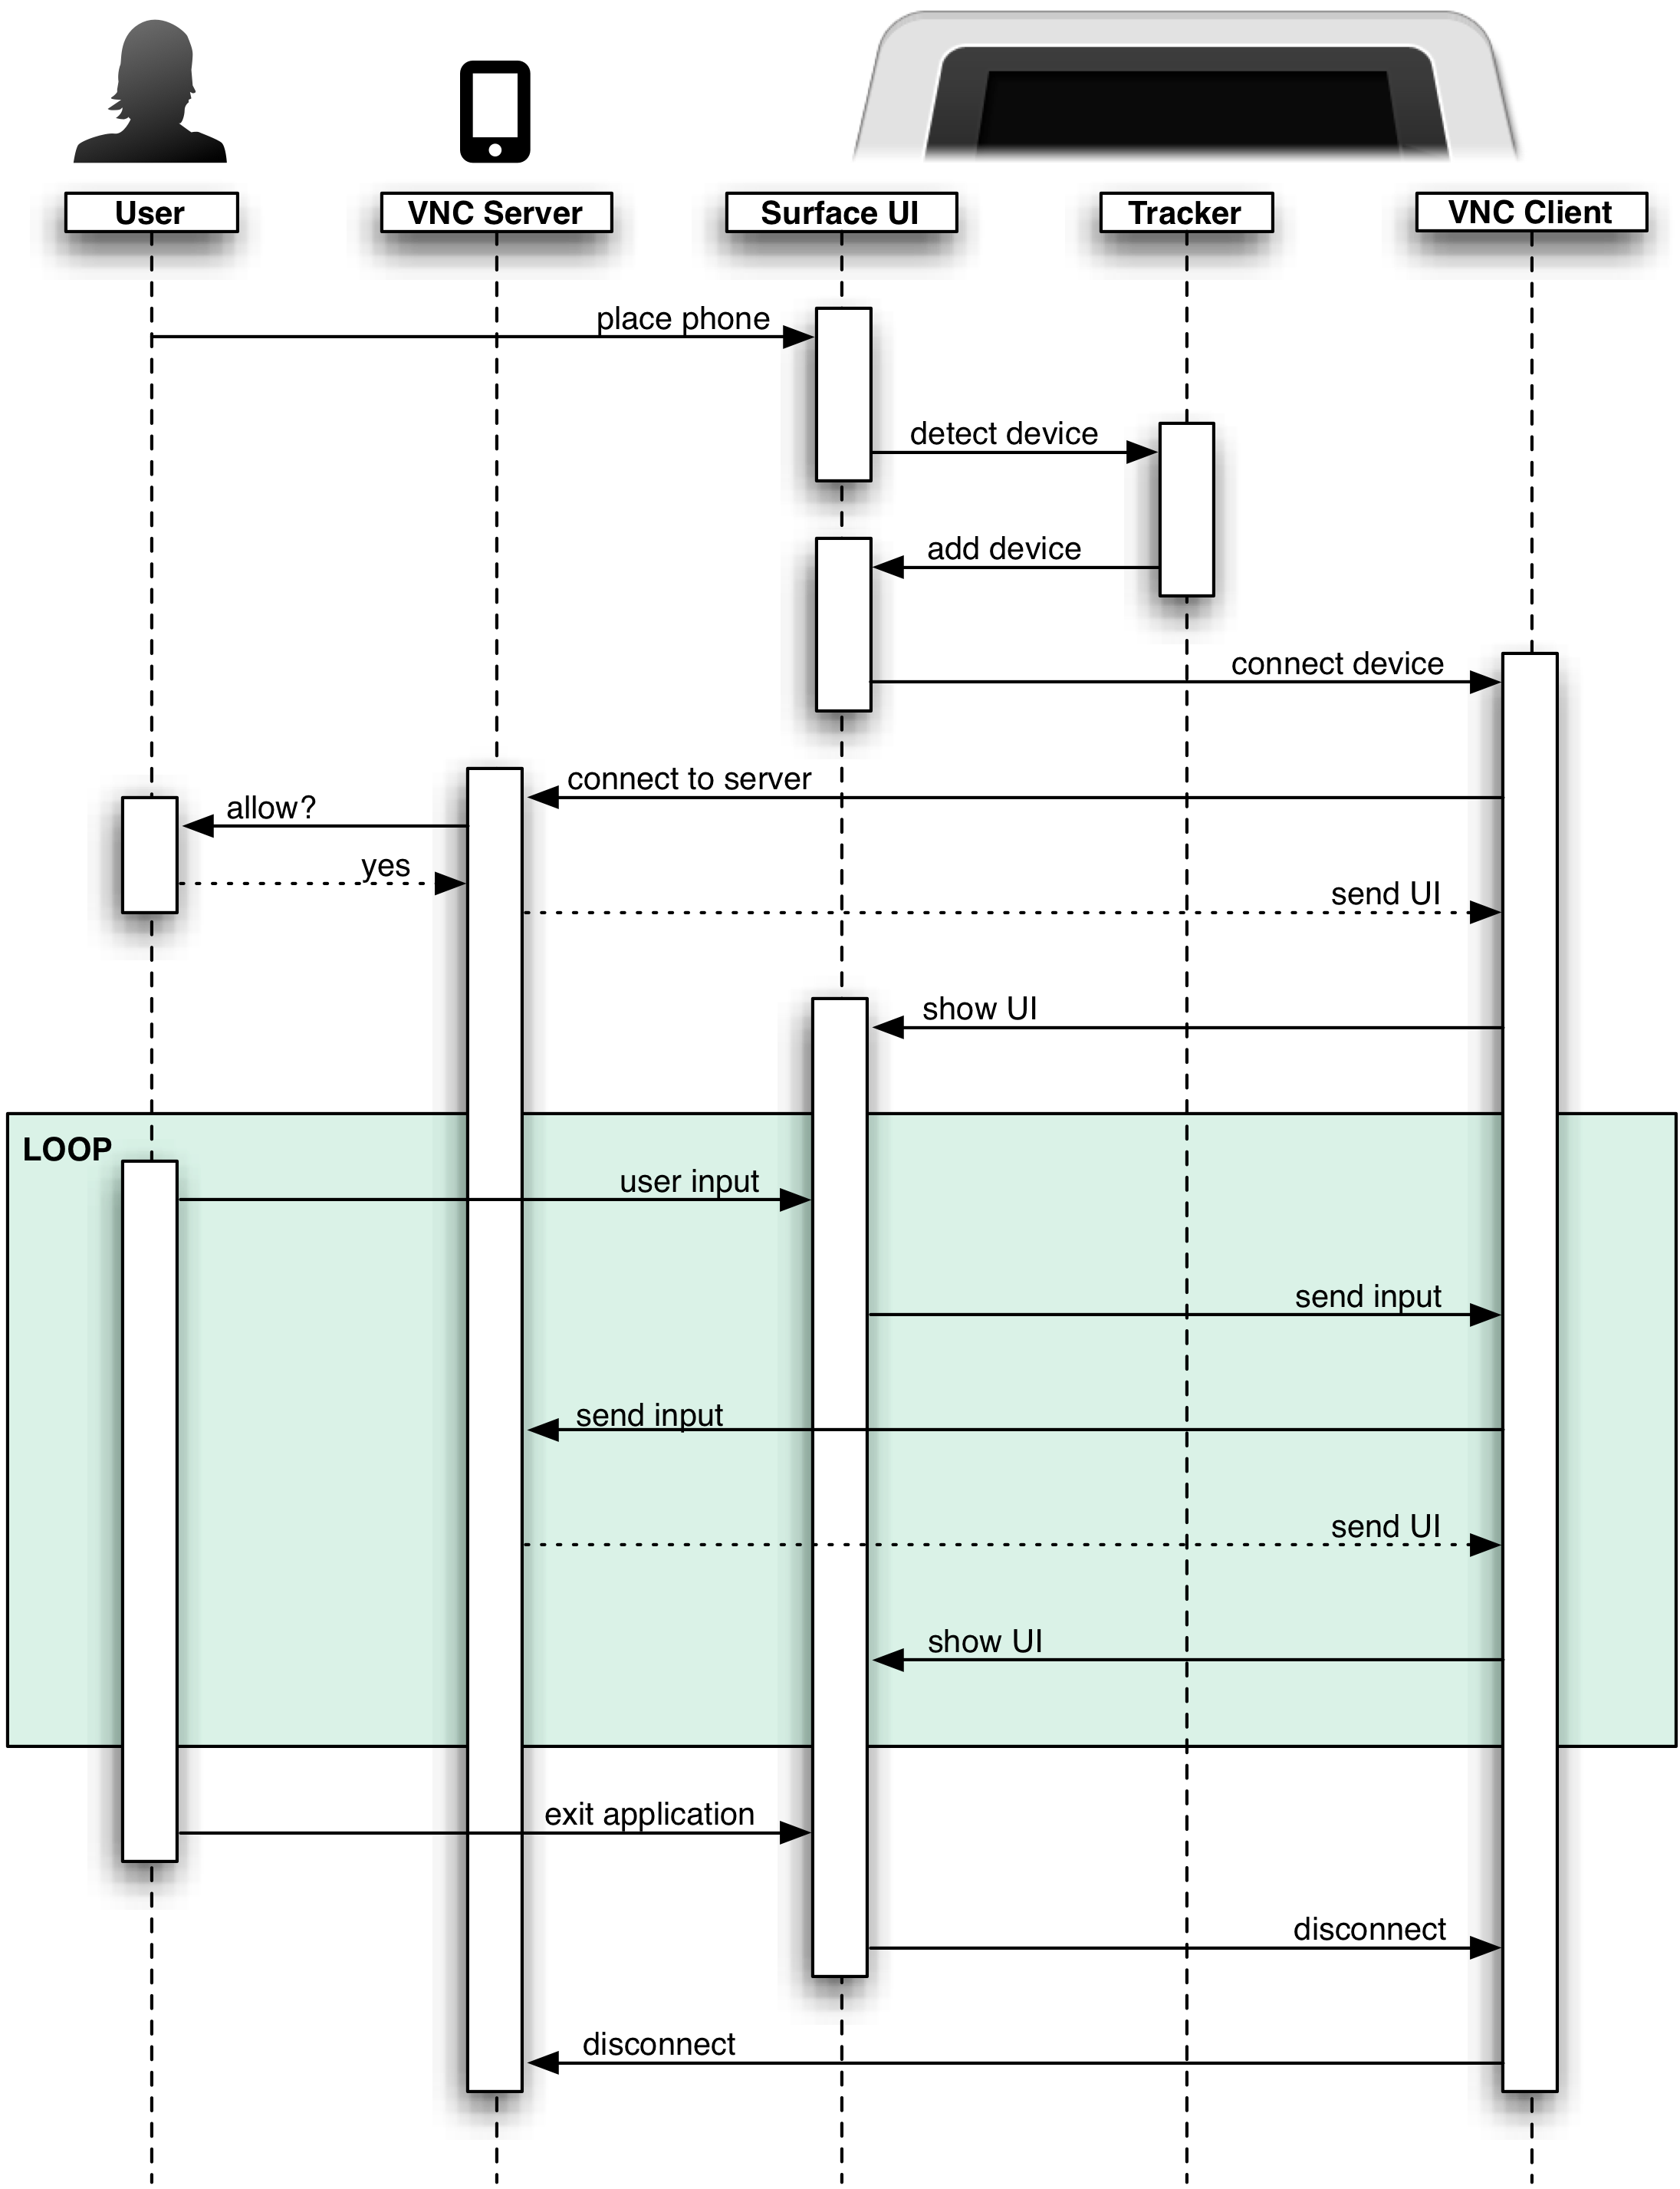
\includegraphics[width=1\textwidth]{images/sequenceOverview}
    \caption{TIDE overview.}
    \label{fig:sequenceOverview}
\end{figure}

\section{Pairing}
\label{sec:pairing}


how it is not new, what are the existing options, what would I recommend in this context. Discussion. How did I solve it and why.

It shows that the pairing procedure can be made quick and easy by using camera-based object detection and wireless connectivity.


\subsection{Vision-based device tracking}
vision-based device tracking
detection options: iPhone App, Tag, camera based 

\begin{figure}[htb]
  \centering
    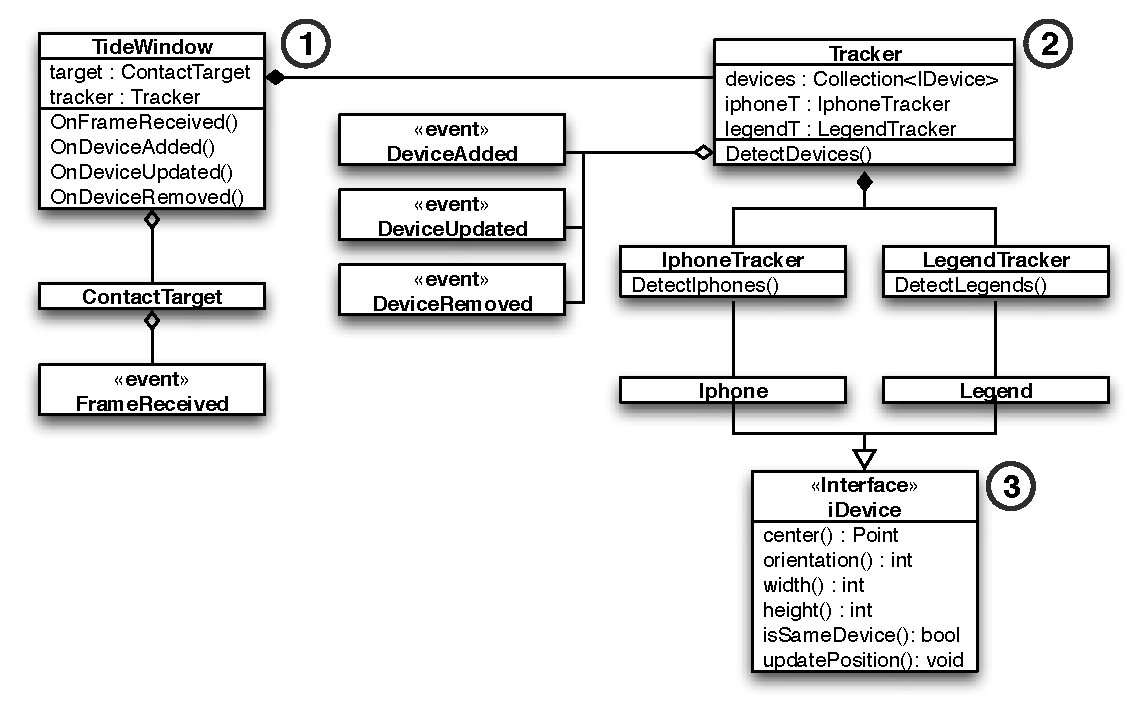
\includegraphics[width=1\textwidth]{images/trackingDiagram}
    \caption{Tracking overview.}
    \label{fig:trackingDiagram}
\end{figure}

\section{Replicated UI}
\label{sec:replicatedui}

 (I/O approach)
- technology issues (slow Veency)

The UI replication is based on the VNC protocol \citep{Richardson:1998:vnc}.

Third-party applications were used on the smartphones, that required rooting the devices.


\section{Surface UI}
\label{sec:surfaceui}

\begin{figure}[htb]
  \centering
    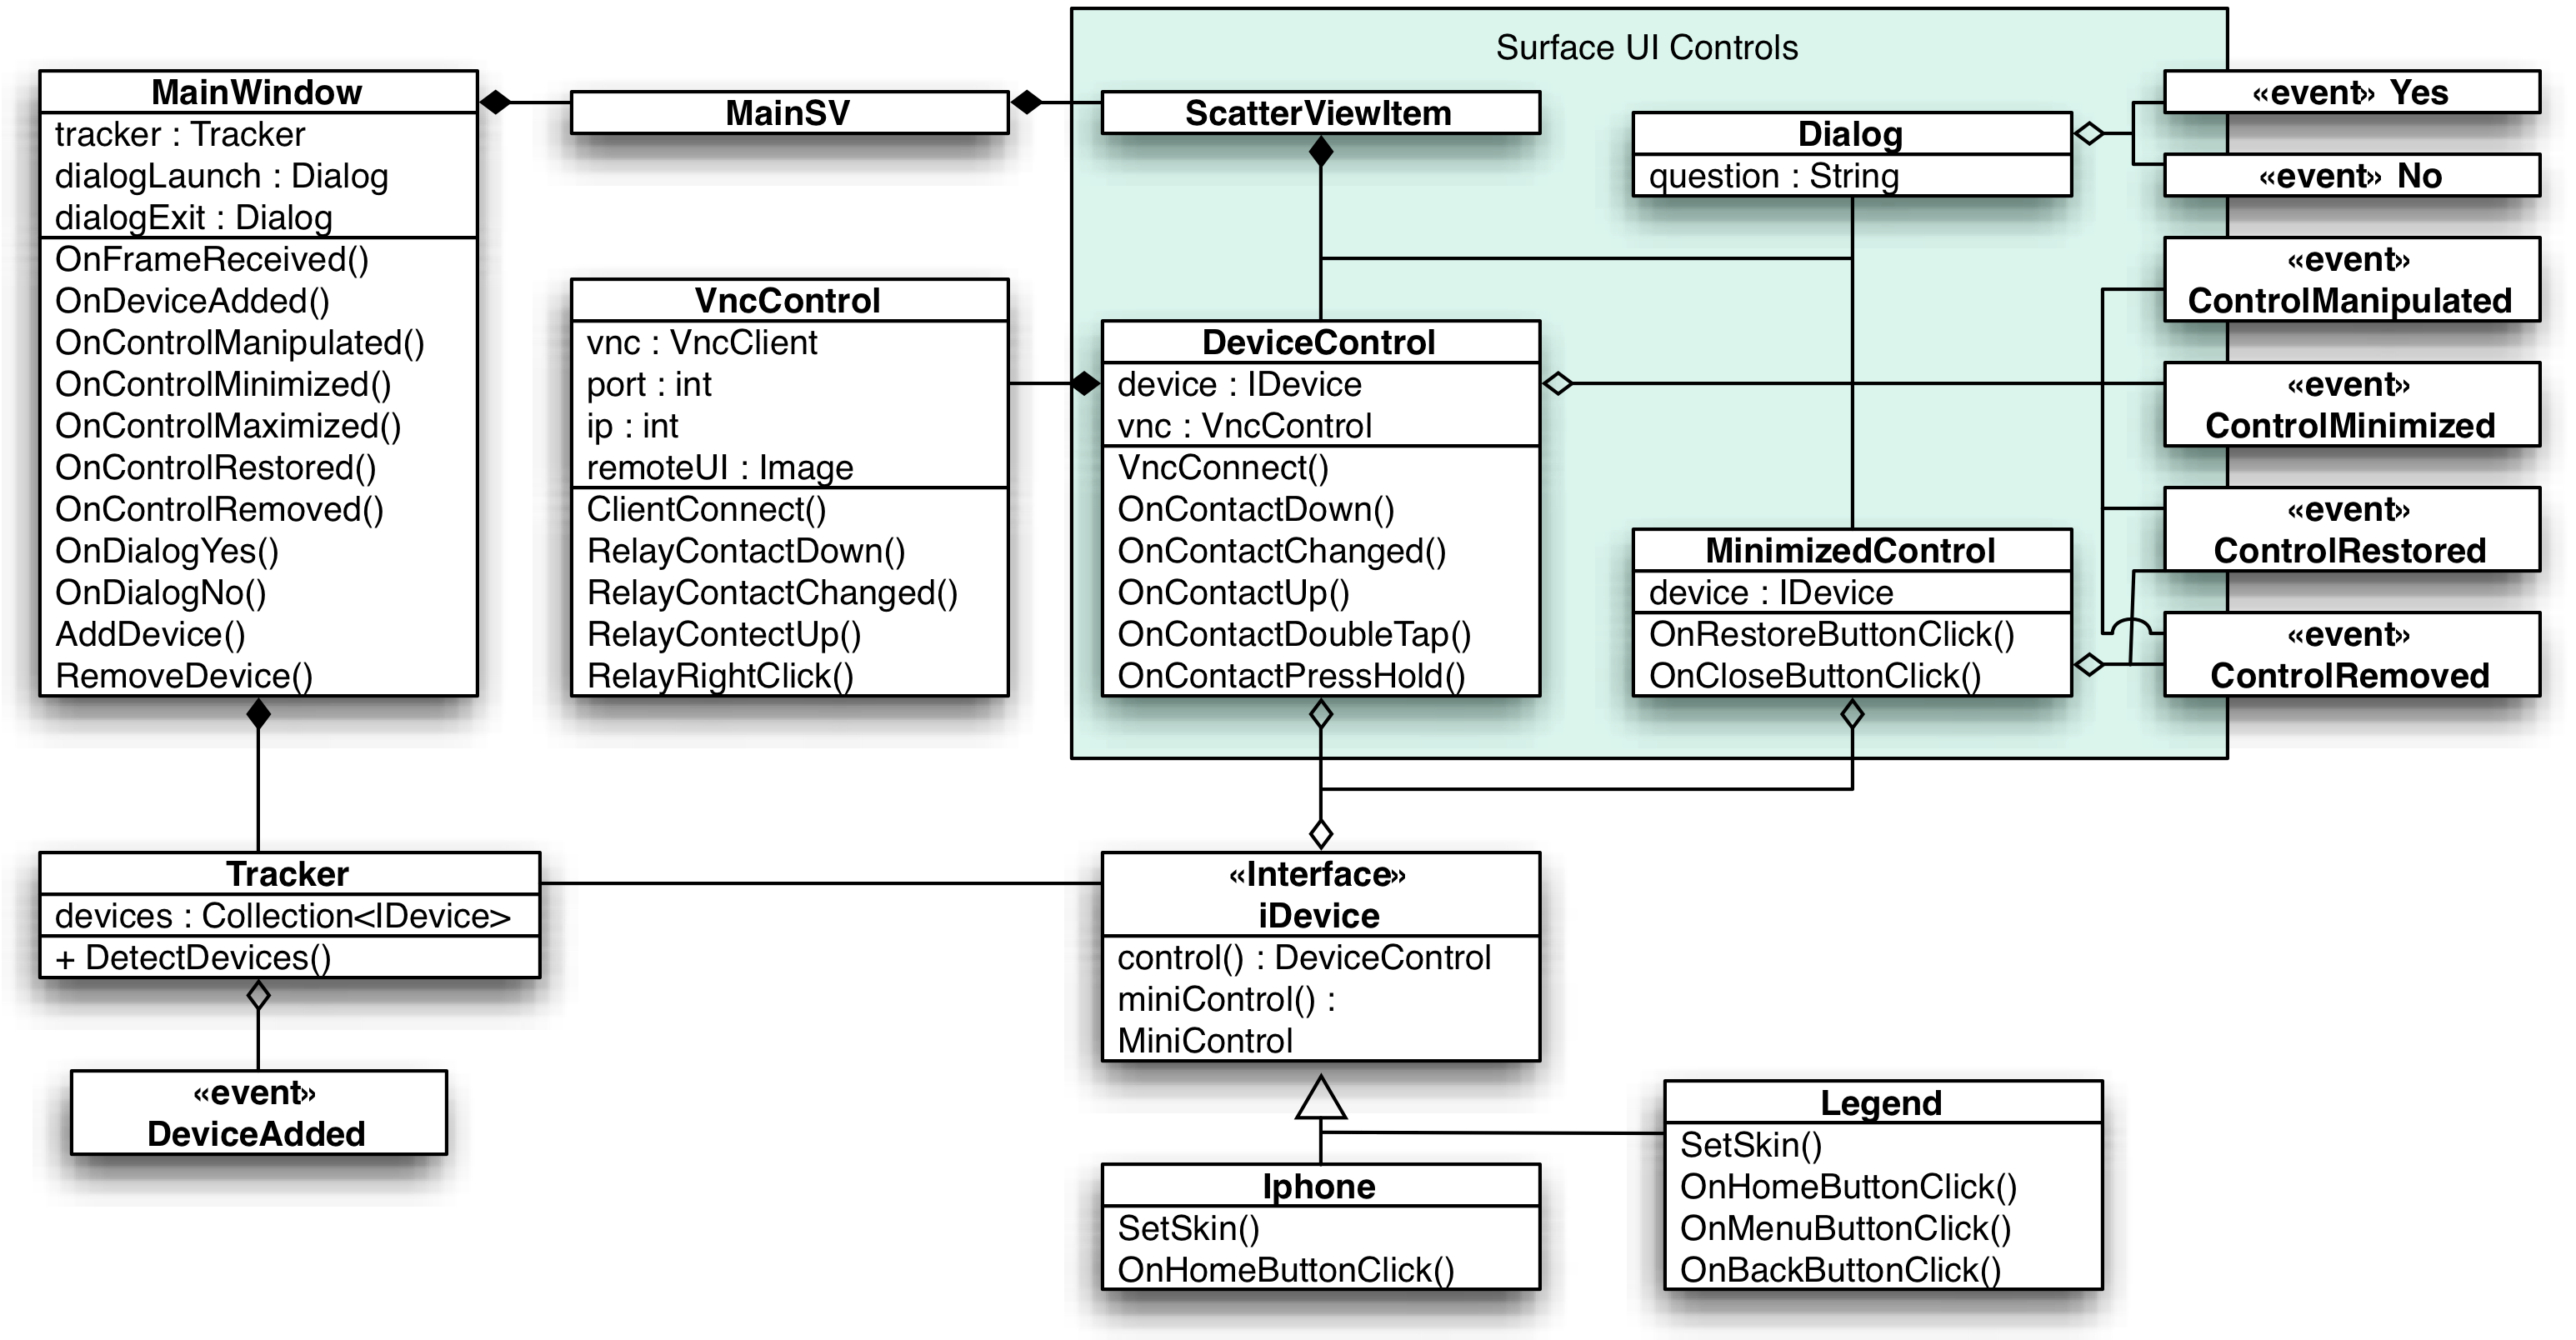
\includegraphics[width=1\textwidth]{images/surfaceDiagram}
    \caption{Surface UI overview.}
    \label{fig:surfaceDiagram}
\end{figure}


\subsection{}

we added MAXIMIZE:
Similarly when enlarged above a certain size, it is maximized to a fullscreen mode. To escape the fullscreen mode, buttons are implemented in the corners of the tabletop.




